% BEGIN TEMPLATE
\documentclass{article}
\usepackage{graphicx}
\usepackage{hyperref} 
\usepackage{xcolor}
\usepackage{nameref}
\usepackage{listings}
\usepackage{float}
\usepackage[title]{appendix}
\graphicspath{ {../../images/} }
% CHANGE THESE
\newcommand{\courseListing}{CSCI 8110-001}
\newcommand{\courseName}{Advanced Machine Learning Applications}
\newcommand{\assignmentTitle}{Homework Assignment \#3}
\newcommand{\assignmentSubtitle}{Attention Modules}
\usepackage{geometry}
\geometry{margin=1in}

\hypersetup{
    colorlinks,
    linkcolor={red!50!black},
    citecolor={blue!50!black},
    urlcolor={blue!80!black}
}
\urlstyle{same}
\definecolor{codegreen}{rgb}{0,0.6,0}
\definecolor{codegray}{rgb}{0.5,0.5,0.5}
\definecolor{codepurple}{rgb}{0.58,0,0.82}
\lstdefinestyle{mystyle}{
    commentstyle=\color{codegreen},
    keywordstyle=\color{magenta},
    numberstyle=\tiny\color{codegray},
    stringstyle=\color{codepurple},
    basicstyle=\ttfamily\footnotesize,
    breakatwhitespace=false,         
    breaklines=true,                 
    captionpos=b,                    
    keepspaces=true,                 
    numbers=left,                    
    numbersep=5pt,                  
    showspaces=false,                
    showstringspaces=false,
    showtabs=false,                  
    tabsize=2
}

\lstset{style=mystyle}

\begin{document}
  \begin{center}
  
\includegraphics[scale=0.15]{UNO-Logo-Color.png}
  \\[0.3in]
  \textbf{\courseListing{}}\\
  \courseName{}
  \\[0.75in]
  \textbf{\assignmentTitle{}}\\
  \assignmentSubtitle{}
  \\[0.75in]
  \textbf{Patrick Davlin}
  \\[0.75in]
  \textbf{Computer Science Department}\\
  \textbf{Peter Kiewit Institute}\\
  \textbf{University of Nebraska}
  \\[0.75in]
  \textbf{Fall 2020}
  \\[0.3in]
  
\includegraphics[scale=0.075]{UNO-Icon-Color.png}
  \newpage
\end{center}
  \graphicspath{{./images/}}
% END TEMPLATE

\section{Project Setup}
\par Previous assignments were developed and executed using the Paperspace Gradient service.
Unfortunately, Gradient recently instituted an \$8 monthly charge, \textit{plus} an hourly charge to use some types of machines.
With this in mind, the work for this assignment was completed using the Google Colab Pro service at its flat \$9 monthly charge.
A static version of the notebook can be accessed by clicking on \href{https://colab.research.google.com/drive/1pp5azAPubxAZP9u5DPgnywmt1fpxQWaU}{this link}.


\section{Process \& Results}
\subsection{Method Selection}
In approaching this project, the first step was to try and gain more familiarity on the concepts of attention modules as described in the course lectures and various academic and research papers.
Given a choice between three types 
Ultimately, the decision of which to implement for this project (only one being required) was arbitrary; the SENet approach was chosen for no reason in particular.
While not a terrifically academic method by which to select a project, it was ultimately somewhat of a coin flip to decide what to implement.

\par To start, a few papers on SENet were consulted. \textbf{[TODO: Complete this section]}
\subsection{Implementation} \label{impl}
\par The first task in implementing this assignment involved determining how best to implement the SENet block as defined in the original paper by Hu, et al \cite{Hu2020Squeeze-and-ExcitationNetworks}.
That model can be found in the figure below:

\begin{figure}[H]
    \centering
    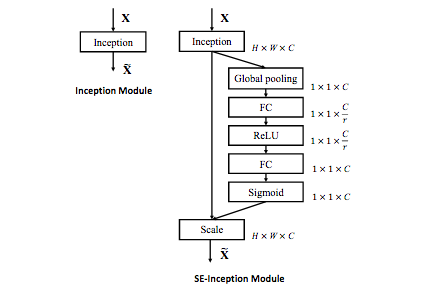
\includegraphics[width=4in]{csci-8110/hw-3/images/SENet_diagram.png}
    \caption{The schema of the original Inception module (left) and the SE-Inception module (right). From Hu, et al \cite{Hu2020Squeeze-and-ExcitationNetworks}.}
    \label{fig:diagram}
\end{figure}

\par Some research had to be done into how to get models to work properly in Keras. 
The format for this SENet block was informed primarily by the method used in the VGG16 source, which can be obtained by Ctrl + Clicking \lstinline{VGG16} in the Google Colab editor.
That format, generally, is as follows:

\begin{lstlisting}[language=Python]
# Block 1
x = layers.Conv2D(
  64, (3, 3), activation='relu', padding='same', name='block1_conv1')(
      img_input)
x = layers.Conv2D(
  64, (3, 3), activation='relu', padding='same', name='block1_conv2')(x)
x = layers.MaxPooling2D((2, 2), strides=(2, 2), name='block1_pool')(x)

# ... and so on
\end{lstlisting}

\par With this in mind, the SENet implementation as defined in Figure \ref{fig:diagram} was, relatively straightforwardly, implemented in code as follows:

\begin{lstlisting}[language=Python]
def SENet_impl(init, ratio=16):
  channel_axis = 1 if K.image_data_format() == "channels_first" else -1
  filters = init.shape[channel_axis]
  se_shape = (1, 1, filters)

  x = GlobalAveragePooling2D()(init)
  x = Reshape(se_shape)(x)
  x = Dense(filters // ratio, activation='relu', kernel_initializer='he_normal')(x)
  x = Dense(filters, activation='sigmoid', kernel_initializer='he_normal')(x)

  if K.image_data_format() == 'channels_first':
    x = Permute((3, 1, 2))(x)

  out = multiply([init, x])
  return out
\end{lstlisting}

\par A significantly more difficult task included getting the SENet implementation included in various locations of the VGG16 model, compiling the new model, training only the relevant layers,and finally getting predictions out of that model once it was compiled.

\subsection{Model Observations}
\par Given that the Keras Vis library makes implementing Grad-CAM so straightforward, it was easy to understand, by inputting different images, how the model isolates features to determine what objects an image contains.
In the case of Jeb, the model does not correctly identify him as a cat.
For Oscar the dog, the model is \textit{much} more reliable:



% \par For stock images, the model is extremely reliable:

% \begin{figure}[H]
%     \centering
%     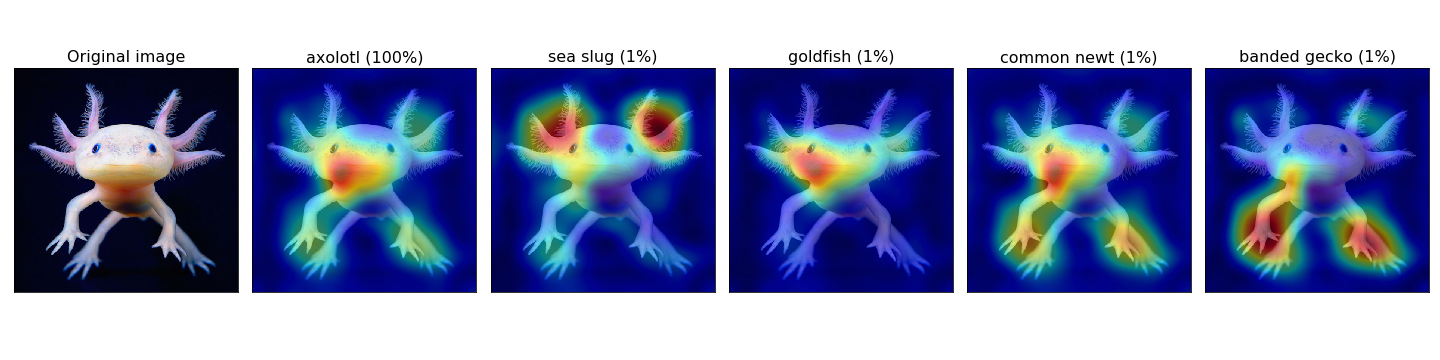
\includegraphics[width=6in]{csci-8110/hw-2/images/axolotl_output.png}
%     \caption{An axolotl}
%     \label{fig:axolotl}
% \end{figure}

\par With the Grad-CAM heatmaps, being able to see the features that each category is "looking" at, is useful for identifying which attributes that the VGG16 model is using to identify an image, given a category.
This is even useful in situations, like with Jeb, where the model has room for refinement.

\par Ideally, the \lstinline{tf-keras-vis} library would have more room for experimentation, or this assignment would have been started with more time to fully implement a Grad-CAM implementation.
In either case, more could be done to visualize the impact of selected layers on the final heatmap.
All said, though, being able to understand the process that models use to identify images is a useful exercise.

\section{Conclusions}
One of the interesting traits of the CAM methods used in this project is that, as a visualization tool, the effectiveness of methods is predicated heavily on a well-trained model.
In practice, this meant that stock images of, say, a goldfish were easily recognizable by the model, where personal photos of a cat were misinterpreted.
Since the results of CAM mapping are tied so closely to that model, and since the process of training models currently feels somewhat out of view, it bears noting that an area of interest for future work might be around training and implementing more training for datasets. It was difficult to resist the urge to try and implement a more robust model for, say, a family member's pet. 
The possibility of doing that kind of work later in this course (or in future academic work) is attractive in that it would provide further opportunities to build an understanding of how neural networks can be supplied with better information on which to make inferences about data.

\par As it stands, though, this project was useful in terms of helping to develop a better understanding of how CNNs can be applied to explain the criteria upon which a trained model perceives input data to be one category (over another).
Being able to use provided Keras tools to implement this made for a somewhat easy assignment; this was so much the case that it felt somewhat uncomfortable writing only a few lines of code for submission.
The foundation provided by Assignment 1 and this assignment should be adequate to move on to more complex topics like training models to data or doing more robust image recognition.

\begin{appendices}

\newpage
\section{Model Output Listing} \label{modelouts}
% \begin{figure}[H]
%     \centering
%     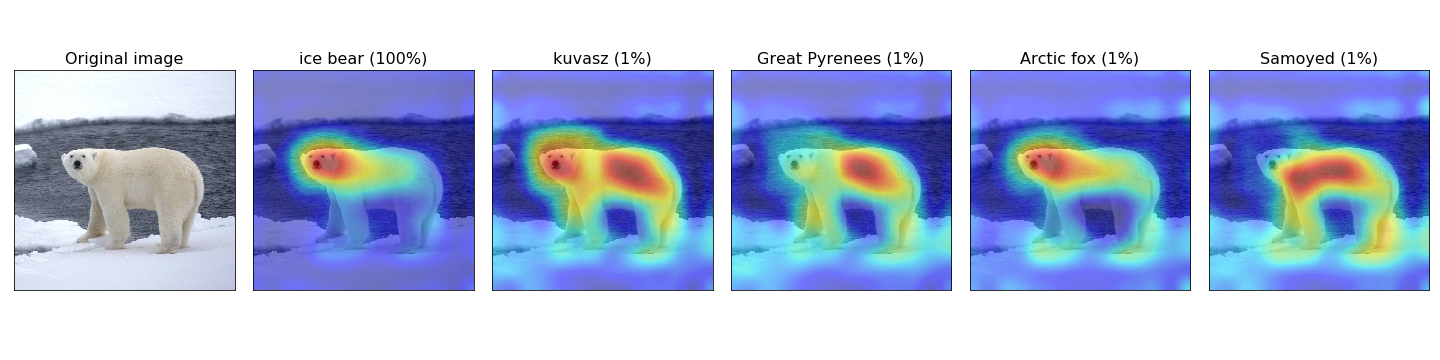
\includegraphics[width=6in]{csci-8110/hw-2/images/bear_output.png}
%     \caption{A polar bear}
%     \label{fig:bear}
% \end{figure}
% \begin{figure}[H]
%     \centering
%     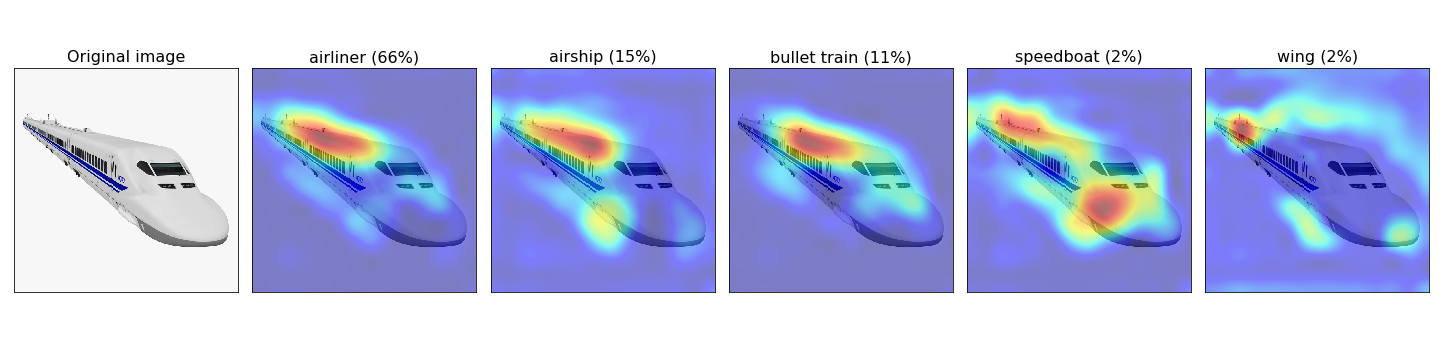
\includegraphics[width=6in]{csci-8110/hw-2/images/bullet_train_output.png}
%     \caption{A bullet train}
%     \label{fig:train}
% \end{figure}
% \begin{figure}[H]
%     \centering
%     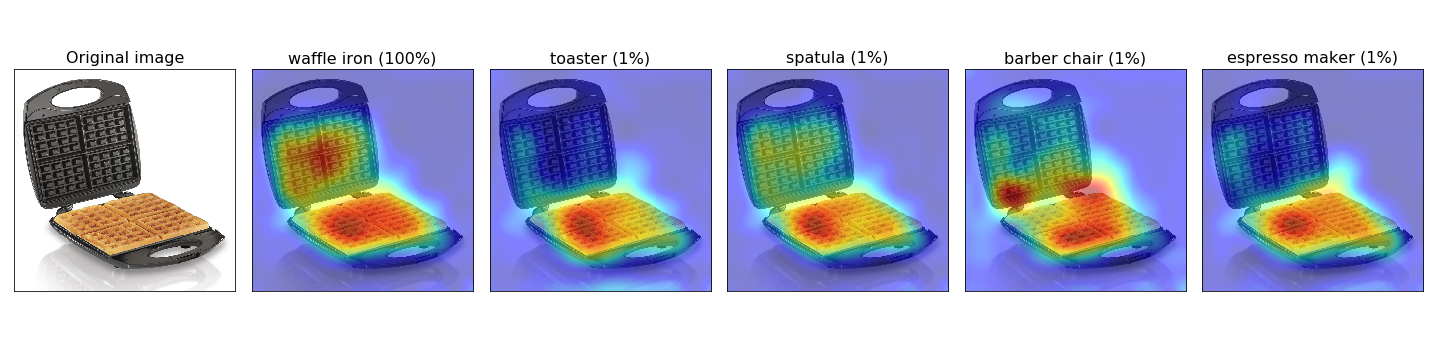
\includegraphics[width=6in]{csci-8110/hw-2/images/waffle_iron_output.png}
%     \caption{A waffle iron}
%     \label{fig:waffle}
% \end{figure}
\newpage
\section{Complete Code Listing} \label{codelist}
% \lstinputlisting[language=Python]{HW2_code.py}
\end{appendices}

\bibliographystyle{unsrt}
\bibliography{references}

\end{document}